\chapter{Giải thuật Deep Sort theo dõi từng người trong khung hình}
Qua các chương trước, luận văn đã trình bày thuật toán, lý thuyết cũng nhhư cách thức hoạt động của chương trình nhận dạng ngôn ngữ ký hiệu. Ở chương này, luận văn sẽ trình bày giải thuật Deep Sort dùng để theo dõi từng người trong khung hình, đánh số thứ tự từng người, cùng với ngôn ngữ ký hiệu của họ muốn diễn đạt.

Phát hiện đối tượng và theo dõi đối tượng là một trong những chủ đề được thị giác máy tính nghiên cứu từ rất lâu. Các thành tựu của chúng đã đạt đến những thành công rất cao cũng như được ứng dụng rộng rãi vào đời sống. Phát hiện đối tượng (objects detection) chỉ tập trung vào việc phát hiện từng đối tượng, đặt chúng trong từng khung hình riêng lẻ và sau đó phân loại đối tượng đó. Việc phát hiện đối tượng chỉ dừng lại ở đây, như vậy đối với cùng một đối tượng nhưng với các khung hình liên tiếp nhau, máy tính sẽ không thể biết được 2 khung hình này chứa cùng một đối tượng . Khác với các thuật toán phát hiện đối tượng, các thuật toán theo dõi đối tượng đều hoạt động theo cách thức khóa từng đối tượng trong khung hình, xác định duy nhất từng đối tượng và theo dõi tất cả chúng cho đến khi chúng rời khỏi khung hình. Ví dụ, nếu máy tính phát hiện được 3 ôtô trong một khung hình, trình theo dõi sẽ phải xác định được 3 đối tượng riêng biệt, đánh số thứ tự chúng và theo dõi qua các khung hình tiếp theo. Theo dõi đối tượng bao gồm theo dõi đối tượng đơn(single object tracking) và theo dõi đa đối tượng (multiple object tracking). Trong phần này, luận văn sẽ chủ yếu đề cập đến các thuật toán theo dõi đa đối tượng cụ thể là giải thuật Deep Sort (được ứng dụng trong luận văn).  
 

\section{Giải thuật Deep Sort}

Phổ biến nhất và là một trong những thuật toán đơn giản nhất để theo dõi là Deep Sort (Simple Online and Realtime Tracking \cite{bewley2016simple}). Thuật toán này có thể theo dõi nhiều đối tượng trong thời gian thực nhưng thuật toán chỉ liên kết các đối tượng đã phát hiện trên các khung khác nhau dựa trên tọa độ của kết quả phát hiện, như hình \ref{fig:sort}

\FloatBarrier
\begin{figure}[htp]
\begin{center}
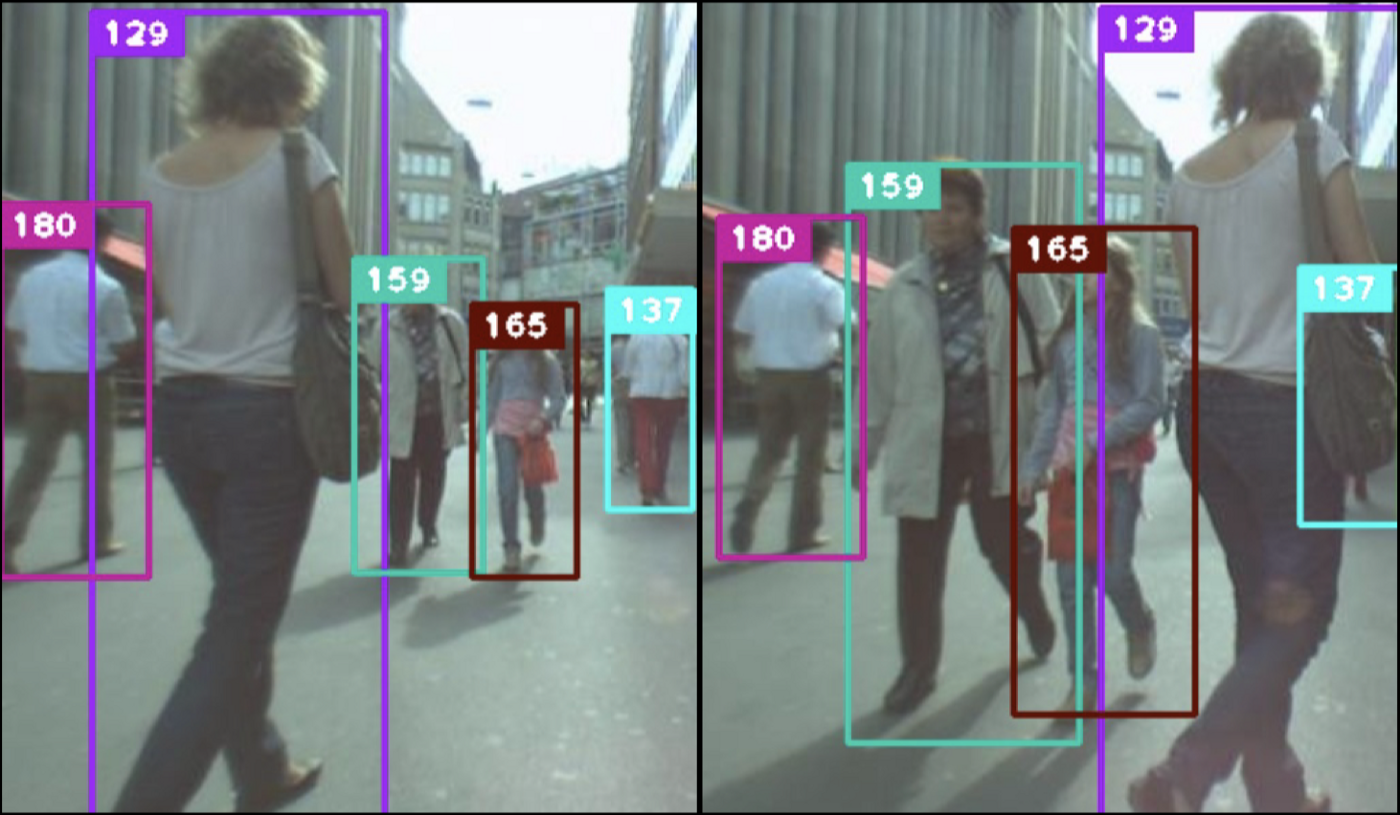
\includegraphics[scale=0.3]{chap5/c5_figs/sort.png}
\end{center}
\caption{Thuật toán Sort\\Nguồn : "Simple Online and Realtime Tracking with a Deep Association Metric" \cite{wojke2017simple}}
\label{fig:sort}
\end{figure}
\FloatBarrier

\section{Kết quả}
Áp dụng giải thuật Deep Sort, luận văn đã theo dõi và đánh số thứ tự được những người có trong khung hình.
\FloatBarrier
\begin{figure}[htp]
\begin{center}
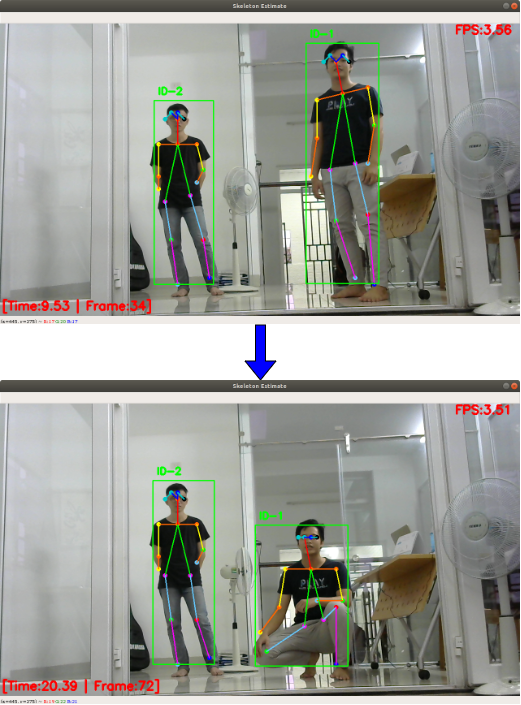
\includegraphics[scale=0.8]{chap5/c5_figs/deep_sort.png}
\end{center}
\caption{Kết quả Deep Sort}
\label{fig:deep_sort}
\end{figure}
\FloatBarrier